\emph{Здесь описывается реализация, в.т.ч. гиперпараметры и процесс обучения доп. классификаторов.}

\subsection{Энкодер начального приближения латентной оптимизации}
%Возможно этот абзац стоит в переработанном виде кинуть в архитектуру
Чтобы ускорить процесс сходимости латентной оптимизации, в данной работе предлагается использовать гибридный подход. Предлагается обучить дополнительную нейронную сеть-энкодер, которая по входному изображению даст грубое приближение его латентного вектора. Использование данное приближение в качестве начального приближения позволит ускорить роцесс сходимости.

Для предсказания начального приближения латентной оптимизации была обучена сверточная нейронная сеть ResNet.
%почему резнет

Для ее обучения с помощью имеющейся генеративной состязательной сети было сгенерированно $50000$ изображений и соответствующих им латентных векторов.
По входному изображению сеть ResNet обучалась предсказывать его латентный вектор. В качестве функции потерь использован логарифм гиперболического синуса ошибки (\emph{Log-Cosh Loss} \cite{chen2019log}), который является гладким аналогом средней абсолютной ошибки.
%log cosh loss, то что он хорош при обучении вариационных автокодировщиков

Нейронная сеть реализована на  фреймворке PyTorch. Сеть обучалать $20$ эпох методом обратного распространения ошибки с использованием оптимизационного алгоритма Adam.
%график нужен

\subsection{Нейронная сеть для латентной оптимизации}

Генератор $G$ является дифференциируемой по входам нейронной сетью, что позволяет напрямую оптимизировать латентный вектор, минимизируя функцию потерь реконструкции. Этот процесс называется латентной оптимизацией. 

\emph{Нужно поправить обозначения на изображении.}
\begin{figure}[h]
\begin{center}
    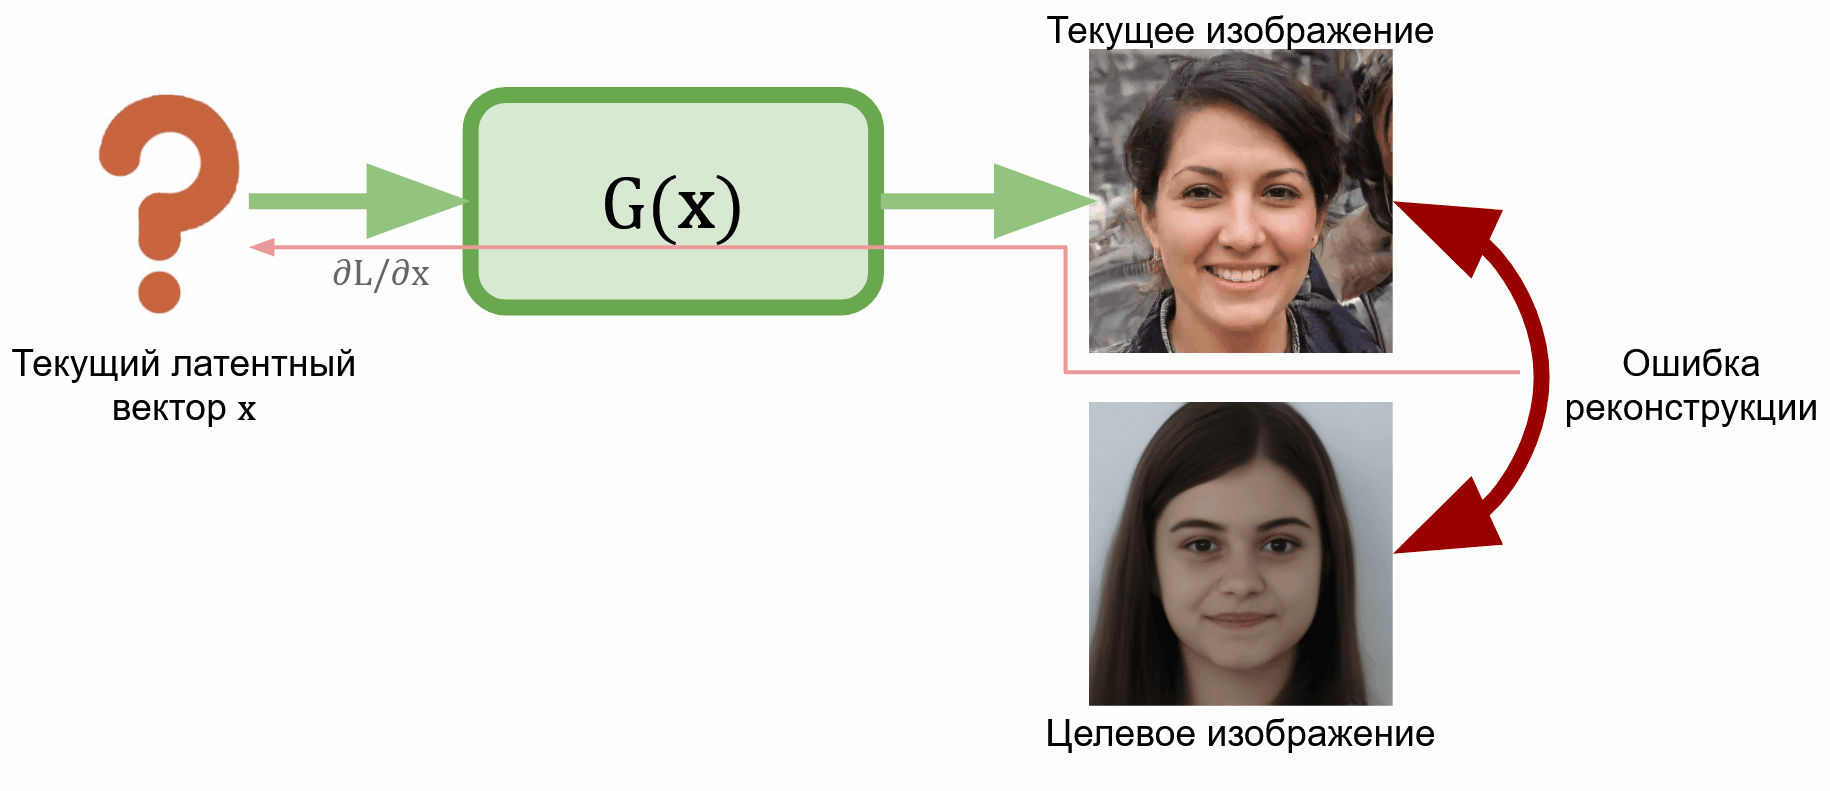
\includegraphics[width=0.9\textwidth]{optim_pipeline_ru}
    \caption{Архитектура нейронной сети для латентной оптимизации}
    \label{fig:optim_pipelin}
\end{center}
\end{figure}

В качестве функцию потерь реконструкции используется взвешенная сумма среднеквадратичной ошибки в пространстве пикселей и визуальной функции потерь (\emph{perceptual loss} \cite{Johnson2016Perceptual}).
%Здесь нужно сказать, что следуем Image2StyleGAN, что используем W+

\emph{Дальше нужно написать достаточно сложный абзац, объясняющий пространство $W+$ и оптимизацию отдельных грубых мап признаков.}
%собственно здесь описываем модификацию того, что ступенчато оптимизируемся и что это позволяет не улететь датеко от данных (см. Latent Space Oddity).

%\subsection{Алгоритм выделения семантик}

\subsection{Алгоритм переноса лицевых признаков с изображения образца}

%Переформулировать в терминах оптимизации.
% Мы оптимизируем пока не сойдемся по одному Degree of Freedom, и при этом делаем ортогональный шаг по остальным Degree of Freedom.
На генерируемом изображении $g(\mathbf x + \alpha \mathbf n)$, полученном путем линейного сдвига в направлении полученного вектора $\mathbf n$, выбранный семантический признак будет более выражен при $\alpha > 0$, и менее выражен при $\alpha  < 0$.

%собственно здесь описываем модификацию того, что используется Face Model для введения нелинейности и сохранения личности.